\documentclass[11pt]{article}
\usepackage[a4paper,margin=22mm,headheight=16pt]{geometry}
\usepackage{fontspec,xeCJK,xcolor,graphicx,enumitem,fancyhdr,titlesec}
\usepackage{hyperref}
\IfFontExistsTF{Times New Roman}{\setmainfont{Times New Roman}}{\setmainfont{TeX Gyre Termes}}
\IfFontExistsTF{FangSong}{\setCJKmainfont[AutoFakeBold=2]{FangSong}}{\IfFontExistsTF{仿宋}{\setCJKmainfont[AutoFakeBold=2]{仿宋}}{\IfFontExistsTF{FandolFang-Regular.otf}{\setCJKmainfont[AutoFakeBold=2]{FandolFang-Regular.otf}}{\setCJKmainfont{FandolSong-Regular.otf}}}}
\definecolor{ink}{HTML}{173747}\definecolor{accent}{HTML}{227E82}
\hypersetup{colorlinks=true,urlcolor=accent,linkcolor=accent}
\linespread{1.22}\setlength{\parindent}{0pt}\setlength{\parskip}{6pt}
\setlist[itemize]{leftmargin=1.4em,itemsep=3pt}
\titleformat{\section}{\large\bfseries\color{ink}}{}{0pt}{}
\titlespacing*{\section}{0pt}{14pt}{7pt}
\pagestyle{fancy}\fancyhf{}\lhead{\small OMNI LEARNING / 学习手册}\rhead{\small Source-grounded learning}\cfoot{\small\thepage}
\emergencystretch=2em\widowpenalty=10000\clubpenalty=10000
\newcommand{\Needspace}[1]{\par\begingroup\dimen0=#1\relax\vskip0pt plus\dimen0\penalty-100\vskip0pt plus-\dimen0\vskip\dimen0\penalty9999\vskip-\dimen0\vskip0pt\endgroup}
\begin{document}


{\LARGE\bfseries\color{ink} 能量转换与效率}\par

2026-10-08 | Day03/30 | 阅读 8 分钟 + 练习 3 分钟\par\vspace{6pt}

\Needspace{5\baselineskip}\section*{今日导航}

今天回答：同样完成照明，为什么两套设备的耗电可以不同？目标是分清能量、功率与效率，并能读懂一个简单用电估算。先回想昨日“测试条件”的问题：使用时长是否也属于必须说明的条件？

\Needspace{5\baselineskip}\section*{沿着能量流观察}

看图 C：阳光被太阳能电池板转换为电能，储能设备保存一部分能量，再供灯具使用。实际装置还需要控制器与电气保护，图中省略了这些部件；不要据图接线。每个环节的输入与输出都可以单独检查，链条上多个转换过程会影响最终可用能量。能源部基础资料把发电、输电与配电分开讨论，也是这种系统观察方式。[S3]

\begin{center}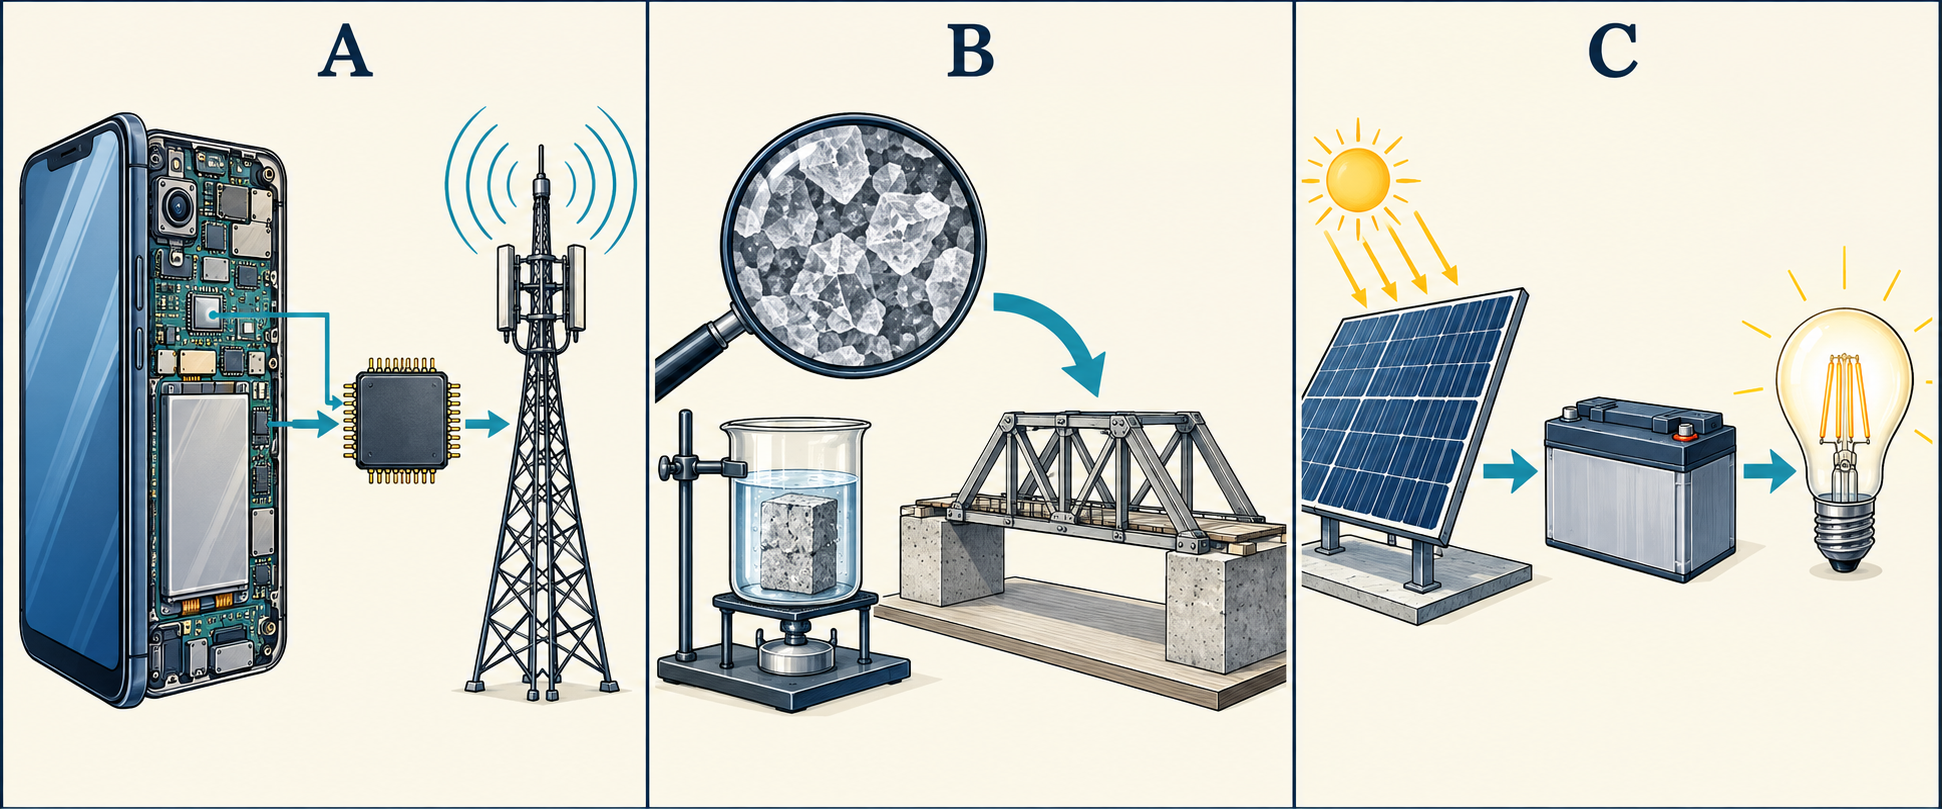
\includegraphics[width=\linewidth,height=0.26\textheight,keepaspectratio]{../assets/figure-f1c69576c177.png}\par

{\small 本课重点看 C 区。A 用手机观察部件与网络；B 区分解释与设计；C 追踪太阳能、储能和照明之间的能量流。箭头为概念关系，不是接线图。}\par

{\footnotesize AI生成教学示意，非实物照片、原始史料或官方架构。生成方式：内置文生图；提示词见仓库 docs/image-prompts.json。}\end{center}

\Needspace{5\baselineskip}\section*{三个容易混淆的量}

能量描述做功或发生变化的能力；功率描述能量转换或使用的快慢。对稳定功率的简化情形，能量等于功率乘时间。家用账单常用千瓦时计量一段时间的用电量，不能把“千瓦时”误读成功率。[S3]

效率关注有用输出占输入的比例。把什么算“有用”取决于任务：电暖器放出的热是目标，照明设备产生的热通常不是照明目标。比较效率时必须比较同一种输出要求，不能只看设备铭牌功率。如果一个灯照度不够，耗电低也未必完成了同样任务。

能量守恒不等于能量都能继续按原用途利用。转换中的热向环境散去后，仍是能量，但要重新集中并转成有用输出并不容易。今天不做热力学推导，只保留这个区别：总量守恒和实际可用性是不同问题。

\Needspace{5\baselineskip}\section*{算一个透明的教学案例}

假设两盏灯提供相同的目标照明，功率分别为10 W和20 W，每天都开5小时。前者一天用电0.05 kWh，后者0.10 kWh；连续30天分别为1.5和3 kWh。这里忽略亮度衰减、待机与电价变化，数字只用于教学，不代表市场上任何产品。

若20 W的灯只开1小时，它的总用电反而低于10 W灯开5小时。可见比较设备与比较实际账单需要不同条件。太阳能系统还要看日照、负载时段和储能损耗；只看电池板峰值功率不能直接推出每天发多少电。

\Needspace{5\baselineskip}\section*{三分钟练习与自查}

一台假想设备稳定功率为50 W，每天运行2小时。估算七天用电，再指出两个现实中可能让估算偏离的原因。

参考：50×2×7=700 Wh，即0.7 kWh。原因可以是功率随负载变化、实际运行时长不同、另有待机消耗。请检查单位有没有跟着换算：1000 Wh才是1 kWh。若你写了电费，还必须说明电价；本题没有给电价，因此无需猜测。

\Needspace{5\baselineskip}\section*{复盘与下一步}

能量看总量，功率看速度，效率看指定任务下的有用输出比例。把这些量放回系统，才能理解技术改善究竟发生在哪里。明天转向材料：为什么同样的设计换一种材料，性能、制造成本和使用寿命都会变化？

\Needspace{6\baselineskip}\section*{扩展学习 / Further reading}\small 以下为选读，不计入每日必做时间。\begin{enumerate}[leftmargin=1.6em]

\item [S1] \href{https://openstax.org/books/physics/pages/1-1-physics-definitions-and-applications}{Physics: Definitions and Applications} — 从物理学与技术的关系入手，区分解释自然和解决实际问题。\par OpenStax | 发布：未标注 | 核验：2026-10-08

\item [S2] \href{https://science.nasa.gov/ems/}{The Electromagnetic Spectrum} — 查看波谱教学材料，理解通信与成像共享的物理基础。\par NASA | 发布：未标注 | 核验：2026-10-08

\item [S3] \href{https://www.energy.gov/oe/electricity-101}{Electricity 101} — 只读发电、输电、配电与 kWh 的基础解释；历史统计不作当前数据。\par 美国能源部 | 发布：未标注 | 核验：2026-10-08

\item [S4] \href{https://www.nist.gov/ai-measurement-and-evaluation}{AI measurement and evaluation} — 观察准确性之外的可靠性与可解释性维度，为后续技术评估做准备。\par NIST | 发布：未标注 | 核验：2026-10-08

\item [S5] \href{https://www.computerhistory.org/siliconengine/}{The Silicon Engine} — 沿晶体管与集成电路历史观察技术如何通过多项改进进入系统。\par Computer History Museum | 发布：未标注 | 核验：2026-10-08

\end{enumerate}

\end{document}